% General document settings
\documentclass[a4paper,12pt]{article}
\usepackage[T1]{fontenc} 			                  % Needed for fonts
\usepackage[latin1]{inputenc}                   % Needed for signs ���
\usepackage[english]{babel}						          % English word dividing
\usepackage{graphicx}					                  % To include graphic files
\usepackage{amsmath, amsfonts, amssymb}         % Packages to write math
\usepackage[amssymb]{SIunits}                   % To use \unit for SI-enheter
\usepackage{float}                              % To use H position specifier
\usepackage[bookmarks]{hyperref}                % Links to chapters in pdf
\usepackage{url}                                % To use \url
\usepackage{array}                              % To use m{1cm} on tables
\usepackage{changepage}													% Allows for temporary adjustment of side margins
\usepackage{longtable}													% Tables across multiple pages
\usepackage[framed]{mcode}											% To include Matlab code directly

% Graphic stuff
\usepackage{tikz,tkz-tab}                       % Package to draw with in LaTeX
\usetikzlibrary{decorations.pathmorphing}       % To draw foton lines
\usetikzlibrary{decorations.pathreplacing}      % To draw brace {}
\usetikzlibrary{shapes,arrows}                  % To draw arrows in tikz
\usepackage{xcolor}                             % Colors
\usepackage{rotating}                           % To rotate stuff
\usepackage{subfigure}                          % To put figures next to each others
\usepackage{epstopdf}                           % To include .eps figures from Matlab export
\DeclareGraphicsExtensions{.pdf,.jpg,.png,.eps,.bmp} % To write graphic filenames without extensions
\graphicspath{{./images/}{../Matlab/Processed_results/}} % To avoid writing path for every image

% Info about the report
\author{Jon Skarpeteig}
\title{Cryogenic micro-photoluminescence of silicon solar cell materials}
\date{\today}


\begin{document}

% Title page
%\begin{titlepage}
 \thispagestyle{empty}

% \maketitle
 
 \centering
 
 
\includegraphics[width=5cm]{NTNU_engelsk_CMYK}
 
  \vspace{15mm} % Vertikalt mellomrom
 
    \Large
  {\bf{\textsl{Master thesis}}} \\
  
  % Tittel
  \vspace{15mm}          % Vertikalt mellomrom
  \huge
  \textbf{Cryogenic micro-photoluminescence of silicon solar cell materials} \\
  \vspace{4mm}
  \large
  \textbf{by} \\
  \vspace{4mm}
 
  % Forfatter
  \large
  \textbf{Jon Skarpeteig} \\
  \vspace{20mm}

  \large
  \today \\
  \vspace{17mm}
  Supervisors: \\ Helge Weman \\ Arne R�yset \\
  \vspace{15mm} 
  \textsl{Norwegian University of Science and Technology} \\
  \textsl{Department of Electronics and Telecommunications} \\
  
\end{titlepage}

\pagenumbering{roman}

% Abstract
%\begin{abstract}
not ready
\end{abstract}


% Table of contents
\clearpage
%\tableofcontents

\clearpage
%\listoffigures

% Actual text in the report
\clearpage
\pagenumbering{arabic}
\setcounter{page}{1}

%\input{introduksjon}
\clearpage
%\input{spektroskopi}
%\input{tap}


\input{theory}
\clearpage
\section{Experimental}

\subsection{Samples}

\begin{table}[H]
\centering
\begin{tabular}{|c|m{6cm}|c|}
\hline
\textbf{Name} & \textbf{Description} & \textbf{Feedstock} \\ \hline
R6-Q3-210 & Polysilicon, electronic grade, clean feedstock & Siemens process \\ \hline
ES1-Q3-201 & Large amount of P and B, solar grade, dirty feedstock & From Elkem \cite{hystad09} \\ \hline
MH2-Q3-201 & Same as ES1 with added Cr, solar grade, dirty feedstock & From Elkem \cite{hystad09} \\ \hline
\end{tabular}
\caption{Samples}
\label{tab:samples}
\end{table}

\subsubsection{R6-Q3-201}

This sample is from a clean feedstock, with low amount of impurities. B,Al and Fe where measured by Glow-Discharge Mass Spectrometry (GDMS), O and C where measured by Fourier transform infrared spectroscopy (FTIR). 

\begin{table}[H]
\centering
\begin{tabular}{|c|c|c|}
\hline
\textbf{Impurity} & \textbf{ppbw} & \textbf{atoms/cm$^3$} \\
\hline
B & 112.01 & 1.45\cdot10$^{16}$ \\ \hline
Al & 19.48 & 1.0\cdot10$10^{15}$ \\ \hline
Fe & nd & nd \\ \hline
C & 2576 & 2.26\cdot10$^{17}$ \\ \hline
O & 1932 & 8.87\cdot10$^{16}$ \\ \hline 
\end{tabular}
\caption{Impurities in R6}
\label{tab:r6_impurities}
\end{table}

The impurities that are not listed were not analyzed, and are expected to be present in very low levels (tenths of ppbw).

\subsubsection{ES1-Q3-201}

This is a regular solar grade sample which originate from a compensated feedstock from Elkem Solar, from 90\% ingot height. It has been Sopori etched to bring out dislocations \cite{soporietch}.

Boron contaminants appear to be between 550 and 700~ppbw, which is between 7.1\cdot$10^{16}$ and 9.7\cdot$10^{16}$~atoms/cm$^3$ respectively using \ref{eq:ppbw}. Phosphorus is measured around 1200-1500~ppbw, which is 5.4-6.8\cdot$10^{16}$~atoms/cm$^3$.
Aluminum contaminants is just below 2.6\cdot10$^{15}$~atoms/cm$^3$. Other contaminants like Ti and Fe have very low values: less than 1.2\cdot$10^{14}$ and 3.8\cdot$10^{14}$~atoms/cm$^3$ respectively. For the lighter atom impurities, O have 1.7\cdot10$^{17}$~atoms/cm$^3$ and C have $6*10^{17}$~atoms/cm$^3$ \cite{hystad09}.

\subsubsection{MH2-Q3-201}

This sample is almost identical to ES1, but the sample also have extra chromium added. Chromium contaminants appear to be between 2 and 5 ppbw \cite{hystad09} which corresponds to 5.4\cdot$10^{13}$ and 1.3\cdot$10^{14}$~atoms/$cm^3$ respectively using \ref{eq:ppbw}, but exact concentration might be a little lower due detection limit of the instrument.


\subsection{Setup}


\begin{figure}[H]
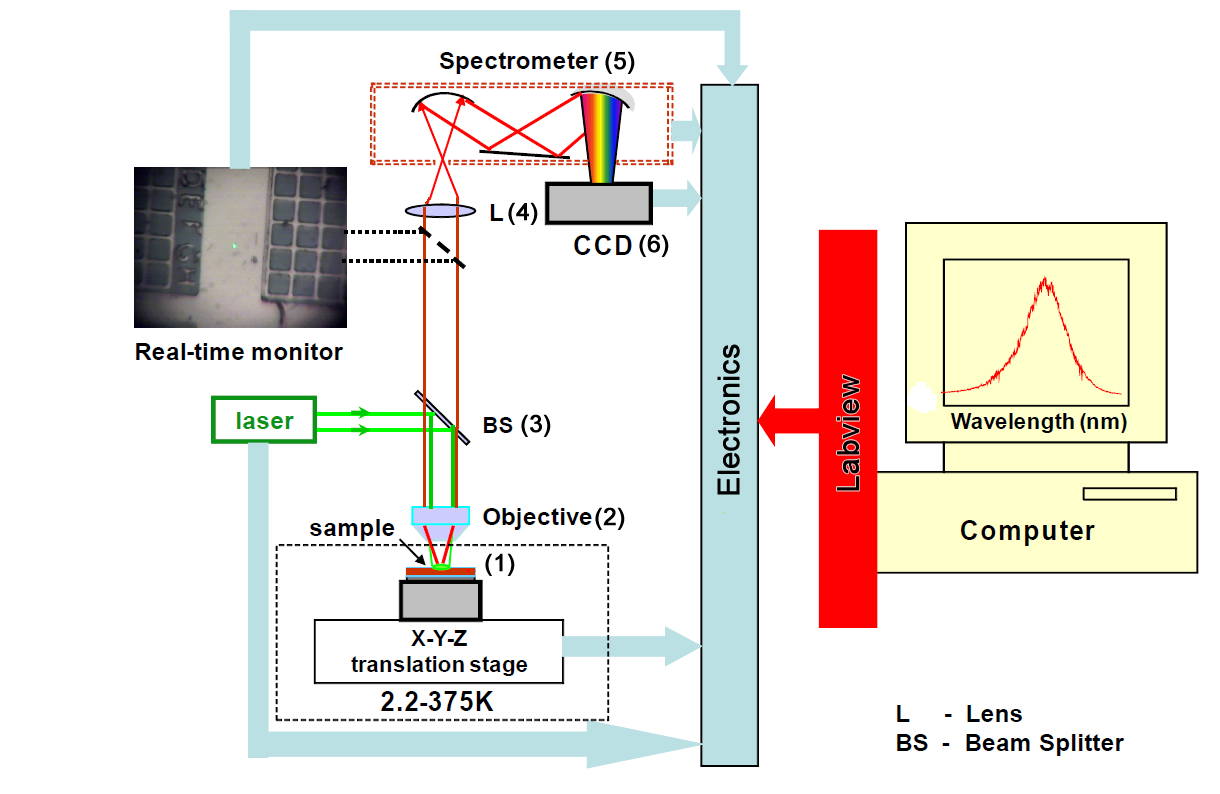
\includegraphics[width=\columnwidth]{lab_setup}%
\caption{Lab setup}%
\label{fig:lab_setup}%
\end{figure}



\begin{table}[H]
\centering
\begin{tabular}{|c|c|c|c|}
\hline
\textbf{\#} & \textbf{Part} & \textbf{Product \#} & \textbf{Manufacturer} \\
\hline
1 & Cryostat & Janis ST-500 & Janis Research Company \\ \hline
2 & Objective & NT56-982 & Edmund Optics \\ \hline
3 & Beam splitter & BS017 & Thorlabs \\ \hline
4 & Lens & ACN127-020-B & Thorlabs \\ \hline
5 & Spectrometer & iHR550 Imaging Spectrometer & Horiba Scientific \\ \hline
9 & Camera & InGaAs Spectroscopy CCD & Andor Technology \\ \hline
\end{tabular}
\caption{Lab setup optical components}
\label{tab:lab_setup}
\end{table}

\subsection{Pumping wavelength}

Pumping light needs to have enough energy to fill all available states in the crystal lattice, in order to detect defects and impurities. For silicon, which has a bandgap of around 1.1eV, has most impurity/defect bands below the bandgap. In order to fill these states, the pumping wavelength should be below 1125nm, which corresponds to energies just over 1.1eV.

Silicon has different absorption lengths for different wavelengths. For 1125nm, the absorption depth is nearly 200~$�$m \cite{laserdybde}. Compared to absorption for 532nm, 1125nm reach 200 times deeper into the sample.

Absorption length of about 1~$�$m for 532 nm laser, means that iron precipitates deeper in the sample won't be detected \cite{gundel09}. This limitation might be overcome by an excitation laser with a longer wavelength and absorption length in silicon. \cite{lee09} report that small angle grain boundaries in multicrystalline silicon of 1$^\circ$-1.5$^\circ$ show D3 and D4 lines, while 2$^\circ$-2.5$^\circ$ show D1 and D2 lines. Comparing to data from electron beam induced current measurements show D1 and D2 lines to be correlated with shallow levels, while D3 and D4 appear in both shallow and deep levels \cite{lee09}.

A pumping wavelength of 800 nm is chosen for excitation. This corresponds to an absorption depth of 12~$�$m in silicon. With a larger wavelength, it would be invisible to the naked eye, and make it much more difficult to align the setup, and make sure nothing is blocking the pathway. In the case of an imperfect filter in front of the spectrometer, 800nm (1.55eV) and the second order diffraction maxima at 1600~nm (0.775~eV) would be outside the most interesting wavelengths from silicon luminescence (see table \ref{energy_bands}).

\subsection{Spot size}

Having a small diameter on the pumping laser allows for a high resolution of characteristics on the sample. In an iron contaminated sample, \cite{gundel09} show that at some distinct spots of a size between 1$�$m and 4$�$m, the band to band photoluminescence peak is particular low at spots with iron precipitates. 

A large electron hole droplet could overshadow characteristics from impurities in the sample. \cite{satoshi04} show that electron hole droplets become more intense for a smaller volume, with a silicon nanolayer smaller than the absorption depth of the laser. \cite{satoshi04} used a 488nm pumping laser with 1,5$�$m diameter, on silicon nanolayer thickness of 50nm and 340nm. For the 50nm layer, \cite{satoshi04} observed a large electron hole droplet, even for small pumping intensities, with the same amount of photo excited carriers per volume as for the 340nm layer. Assuming that a small volume give rise to a larger electron hole droplet, it would be a limiting factor for the spot size and pumping wavelength.

For the setup given here, the spot size is around 2~$�$m.

\subsection{Laser intensity}

With a large pumping intensity, an electron hole droplet become visible in the specter around 1.08eV in bulk silicon \cite{hammond75}. \cite{satoshi04} show that electron hole droplets occur at weak excitations (0.75mW) and even at high temperatures for a silicon nanolayer of 50nm. For thickness of 340nm, the electron hole droplet show up at pumping intensity of 3mW and above, and the intensity of the electron hole droplet grow larger than for the free exciton at 15mW. This electron hole droplet is not wanted, as it can mask characteristic photoluminescence from impurities.

With a larger pumping intensity, the impurity photoluminescence would in some cases also increase. Photoluminescence from chromium bound with a boron atom is known to increase linearly with laser power \cite{conzelmann82,conzelmann83}, and would be easier to detect at a higher pumping intensity.

\subsection{Expected results}

\subsubsection{Phosphorus and boron doped samples}

With fairly high concentrations of doping atoms, it's expected that they show up as separate lines in the photoluminescence spectra. \cite{dean67} observe a line around 1.0924eV which is attributed to B$^{TO}$. Concentrations values for B in \cite{dean67} are $6*10^{16}$~cm$^{-3}$. Also observed is a phosphorus line at 1.0916eV, with 8*10$^{16}$cm$^-3$ phosphorus atoms. ES1 and MH2 have similar B and P values, and is expected to show the same behavior. (See figure \ref{fig:boronSiPL} and \ref{fig:PSiPL} in appendix \ref{appendix:tabeller})

There is a photoluminescence line involving carbon bound to oxygen in Czochralski silicon known as the C-O band \cite{davies88}. In \cite{hare72}, it was observed only in crucible grown silicon, but not in float zone. In the crucible grown silicon, the oxygen impurities where 2\cdot10$^{18}$~atoms/cm$^3$, which is over ten times more than in ES1 and MH2. This makes it unlikely that any C-O complex luminescence will be strong enough to be detectable in these samples.

Another line involving carbon, is the two-carbon atom band \cite{davies88}. This band has been detected in float-zone silicon with C = 9.7\cdot10$^{16}$~cm$^{-3}$ after irradiation, together with the C-O complex line. The relative intensity between the C-O band and the two-carbon atom band in \cite{davies88} show that the 969~meV band is close to 5 times larger than the 789~meV band. With both MH2 and ES1 having carbon impurities around 6\cdot10$^{17}$~cm$^{-3}$ it is possible that this line at 969~meV will be visible. 

As for aluminum, \cite{dean67} show a line at 1.09~eV called Al$^{TO}$ in a sample with 2\cdot10$^{16}$cm$^{-3}$ Al doping atoms. In ES1 and MH2, the Al impurities are 20 times less. In addtion to a fairly low value of Al impurities, the Al$^TO$ line is very close to the I$^{TO}$, which can make it difficult to detect, and not likely to show up in the results.

Fe bound with boron is also known to give rise to photoluminescence \cite{mohring83}. The sample used in the article had  10$^{13}$ to 10$^{16}$~cm$^{-3}$ boron doping concentration. The article doesn't mention how many Fe impurity atoms that's introduced into the sample, but it's done by high temperature diffusion, and assumed to be considerably larger than for all the samples in this study. 

Based on the low values of Fe impurities in these samples, it's assumed that interstitial Fe won't have any effect on the photoluminescence bands. The same goes for Ti, which also have a very low amount present.


\subsubsection{Sample with added Chromium}

This sample have the same impurity values as ES1, except for chromium. The closest comparison is samples used in \cite{conzelmann82}. Here, luminescence spectra was observed for chromium in an p-type sample. Interstitial chromium concentrations where between $10^14$ and $10^16 atoms/cm^-3$ in \cite{conzelmann82}.

Chromium in an n-type sample doped with phosphorus atoms does not result in any luminescence, but chromium bound with boron show a clear line at 0.8432eV (CrB$^0$). The reaction velocity for the formation of CrB pairs at room temperature depend on the boron concentration. For large (10$^15$cm$^-3$) boron content, the chromium-boron reaction reach saturation in less than a day after chromium diffusion \cite{conzelmann82}.

MH2 are neither n og p-type, however there is enough boron atoms to saturate chromium by forming CrB pairs. Chromium atoms are in the order of 10$^{14}$~atoms/cm$^3$ which is similar to that in \cite{conzelmann82}. Expected photoluminescence spectra is therefor expected to be similar. (See figure \ref{fig:CrBSiPL} in appendix). With most of the boron bound with chromium, it is likely that the boron lines will be severely reduced compared to ES1, and not detectable. There are also Fe impurities present in the sample, that can form bonds with boron. Based on the low amount of Fe in this sample, those bonds are not believed to have any impact on the photoluminescence.

\subsubsection{Sample from clean feedstock}

Having carbon values around 2.26\cdot10$^{17}$, it is possible that the two-carbon atom band is visible here also. Else this sample is expected to only show intrinsic values similar to \cite{dean67} in so called "`good"' areas due to low concentration of impurities. However, there might be precipitates and higher concentration of impurities at the grain boundaries and dislocations. Particularly heavy metals like Fe and Al can be detected here. It is expected that the band to band recombination from silicon show considerably lower intensity for these areas.

\subsection{Results plotting}
In order to plot the results from the spectrometer, there are a few manipulations that's needed.

\subsubsection{Disregarding defect pixels}

By taking a spectra with the shutter closed, it is possible to measure the dark current coming from the camera. The dark current should be equally distributed across the pixels, based on the assumption that all pixels behave the same. For long integration time, this is not the case:

\begin{figure}[H]
\centering
\includegraphics[width=\columnwidth]{Dark_current-40s}
\caption[Defective pixels]{Dark current signal from the camera with defective pixels with shutter closed, and CCD at -75$^\circ$C using a random center wavelength}%
\label{fig:dark_current_40s}%
\end{figure}

To solve this problem, the four pixels are disregarded, and the value of the neighbor pixel has been used instead. Matlab code for this is available in the appendix. Comparing the before and after clearly show how this is done:

\begin{figure}[H]
\centering
\includegraphics[width=\columnwidth]{Dark_current-40s_corrected}
\caption[Defective pixels corrected]{Dark current signal from the camera with defective pixel correction in red using a random center wavelength}%
\label{fig:dark_current_40s-corrected}%
\end{figure}

The defective pixels are less apparent for shorter integration time, but still a problem:

\begin{figure}[H]
\centering
\subfigure[Dark current without correction]{
\includegraphics[width=.45\columnwidth]{Dark_current-10s}
\label{fig:dark_current_10s}
}
\subfigure[Dark current with correction (red)]{
\includegraphics[width=.45\columnwidth]{Dark_current-10s_corrected}
\label{fig:dark_current_10s-corrected}
}
\label{fig:dark_current_correction_10s-parentfig}
\caption[Dark current with 10s integration time]{Dark current with 10s integration time using a random center wavelength}
\end{figure}

Dead pixel correction is performed in all results.

\subsubsection{Noise reduction}

As seen in the previous section, there is a dark current offset present. Ideally, all pixels should behave exactly the same, and give rise to the same dark current offset. If all pixels behaved the same, and with the same variance in between measurements, it could simply be subtracted. This is not the case. The dark current is unevenly distributed over the pixel array, and needs to be measured by itself in order to remove it. The mean dark current noise shape is pretty much the same from measurement to measurement using the same CCD temperature. In addition to the mean offset, there is white noise elements. 

\begin{figure}[H]
\centering
\includegraphics[width=\columnwidth]{Dark_current_and_background_noise-20s}
\caption[Dark current and noise]{Dark current (blue) and dark current + background noise (red) with Savitzky-Golay filtered noise floor estimation (cyan)}%
\label{fig:dark_current_and_background_noise}%
\end{figure}

By subtracting the mean offset found in the dark current noise measurement, only background noise and white noise would be left. The matlab code used to do this can be found in the appendix.

\begin{figure}[H]
\centering
\includegraphics[width=\columnwidth]{Dark_current_removed-20s}
\caption[Dark current removed]{Dark current removed from background noise (blue), and Savitzky-Golay filtered signal (cyan)}%
\label{fig:dark_current_removed-20s}%
\end{figure}

It appears that the dark current noise is larger with the shutter open, compared to closed. But a more critical noise in the spectrum is a background signal around 1064nm. The spectrometer has a range of 140nm when using 300 as grating. It has proven difficult to align the system so that the entire array of pixels in the camera get an equally distributed light beam. And based on the noise level, the nm interval is chosen as 100nm, in order to remove the left hand side of the spectra when gluing different intervals together. This also avoid the problem of not hitting the entire array evenly. To get a full overview over the background noise, a full spectra was done, and glued together. This full spectra show that the artifact visible in \ref{fig:dark_current_removed-20s} is the only background noise line visible in the wavelength area 800-1650nm.

\subsubsection{Savitzky-Golay filtering}

Savitzky-Golay filter (also called digital smoothing polynomial filter or least-squares smoothing filter), is a smoothing filter which essentially performs a local polynomial regression on a series of values equally spaced. This filter is chosen because of the large frequency span of the signal. Although Savitzky-Golay filters are more effective at preserving the pertinent high frequency components of the signal, they are less successful than standard averaging FIR filters at rejecting noise \cite{signal_processing}.

\clearpage
\section{Results}

Results have been corrected for dead pixels, measured dark current, and measured background noise unless otherwise specified. Grating is fixed at 300, and pumping wavelength is 800nm. Counts is a number given from the spectrometer which relate to the relative intensity detected by the pixel in the CCD.

\subsection{R6-Q3-210}

This is the electronic grade sample, with a very low amount of impurities.

\begin{figure}[H]
\centering
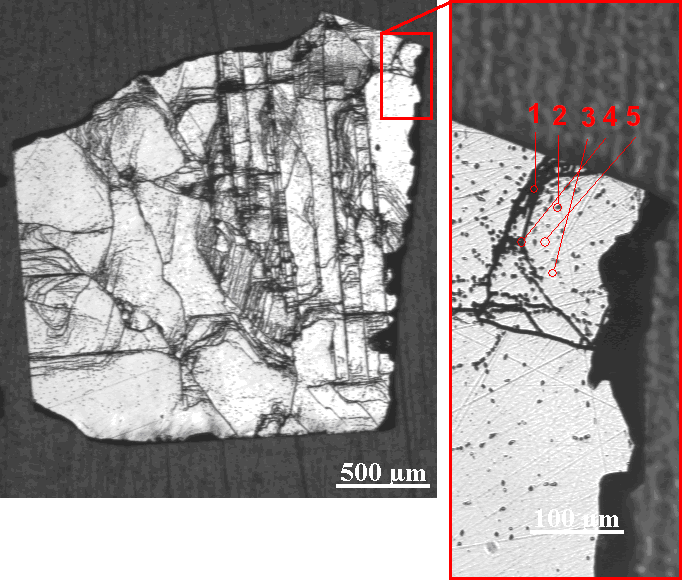
\includegraphics[width=0.7\columnwidth]{R6-Q3-210-A_enlarged}
\caption[R6-Q3-210 A from light microscope]{Sample R6-Q3-210 A picture taken using light microscope. Area 1,2 and 3 are spots where photoluminescence has been measured.}
\label{fig:R6-Q3-210-A_enlarged}%
\end{figure}


\begin{figure}[H]
\centering
\includegraphics[width=0.7\columnwidth]{R6-Area1_dislocation_line-20s}
\caption[R6-Q3-210 at a dislocation line]{Sample R6-Q3-210 A pumped with 170mW at 10K in a dislocation line (Area 1 in figure \ref{fig:R6-Q3-210-A_enlarged}).}
\label{fig:R6-Area1_dislocation_line-20s}%
\end{figure}


\begin{figure}[H]
\centering
\includegraphics[width=0.7\columnwidth]{R6-Area2_dislocation_dot-20s}
\caption[R6-Q3-210 at a dislocation dot]{Sample R6-Q3-210 A pumped with 170mW at 10K in a dislocation dot (Area 2 in figure \ref{fig:R6-Q3-210-A_enlarged}).}
\label{fig:R6-Area2_dislocation_dot-20s}%
\end{figure}


\begin{figure}[H]
\centering
\includegraphics[width=0.7\columnwidth]{R6-Area3_clean_area-20s}
\caption[R6-Q3-210 at a dislocation free area]{Sample R6-Q3-210 A pumped with 170mW at 10K in a dislocation free area (Area 3 in figure \ref{fig:R6-Q3-210-A_enlarged}).}
\label{fig:R6-Area3_clean_area-20s}%
\end{figure}

\subsection{ES1-Q3-201}

This sample is from a dirty feedstock, with large amount of P and B.


\begin{figure}[H]
\centering
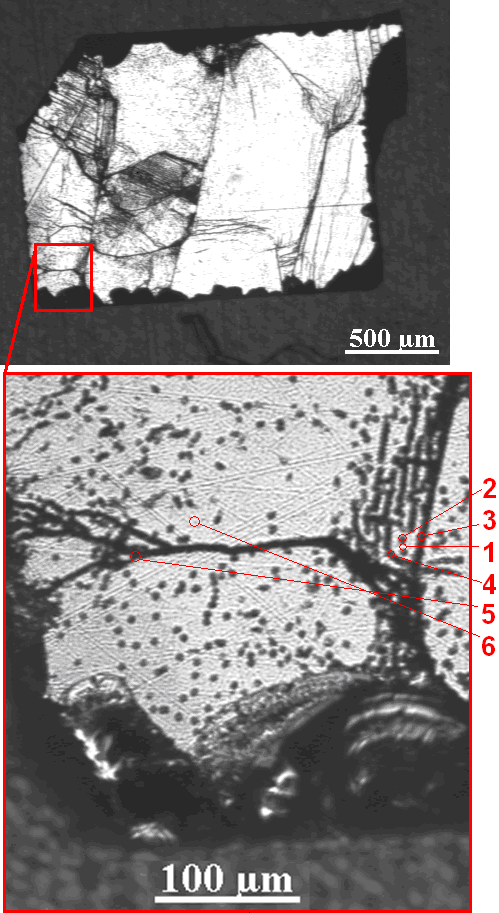
\includegraphics[width=0.85\columnwidth]{ES1-Q3-201-C_enlarged}
\caption[ES1-Q3-201 C from light microscope]{Sample ES1-Q3-201 C 210 A picture taken using light microscope. Area 1,2,3 and 4 are spots where photoluminescence has been measured.}
\label{fig:ES1-Q3-201-C_enlarged}%
\end{figure}

\subsubsection{Room temperature}

\begin{figure}[H]
\centering
\includegraphics[width=0.7\columnwidth]{ES1-room_temperature}
\caption[ES1-Q3-201 at room temperature]{Sample ES1-Q3-201 A pumped with 26mW at 295K in a dislocation line (black) and in a clean area (blue). An estimated dark current offset has been subtracted.}
\label{fig:ES1-room_temperature}%
\end{figure}


\subsubsection{Low temperature}

\begin{figure}[H]
\centering
\includegraphics[width=0.7\columnwidth]{ES1-Area1_dislocation_free-10s}
\caption[ES1-Q3-201 at a dislocation free area]{Sample ES1-Q3-201 C pumped with 170mW at 12K in a dislocation free area (Area 1 in figure \ref{fig:ES1-Q3-201-C_enlarged}).}
\label{fig:ES1-Area1_dislocation_free-10s}%
\end{figure}

\begin{figure}[H]
\centering
\includegraphics[width=0.7\columnwidth]{ES1-Area2_dislocation_spot-10s}
\caption[ES1-Q3-201 at a dislocation free area]{Sample ES1-Q3-201 C pumped with 170mW at 12K in a dislocation spot (Area 2 in figure \ref{fig:ES1-Q3-201-C_enlarged}).}
\label{fig:ES1-Area2_dislocation_spot-10s}%
\end{figure}


\begin{figure}[H]
\centering
\includegraphics[width=0.7\columnwidth]{ES1-Area3_grain_boundary-10s}
\caption[ES1-Q3-201 at a grain boundary]{Sample ES1-Q3-201 C pumped with 170mW at 12K in a grain boundary (Area 3 in figure \ref{fig:ES1-Q3-201-C_enlarged}).}
\label{fig:ES1-Area3_grain_boundary-10s}%
\end{figure}

\begin{figure}[H]
\centering
\includegraphics[width=0.7\columnwidth]{ES1-Area3_grain_boundary_60s}
\caption[ES1-Q3-201 at a grain boundary]{Sample ES1-Q3-201 C pumped with 170mW at 12K in a grain boundary (Area 3 in figure \ref{fig:ES1-Q3-201-C_enlarged}) with the result in figure \ref{fig:ES1-Area3_grain_boundary-10s} plotted as the black line.}
\label{fig:ES1-Area3_grain_boundary_60s}%
\end{figure}


\begin{figure}[H]
\centering
\includegraphics[width=0.7\columnwidth]{ES1-Area4_dislocation_line-10s}
\caption[ES1-Q3-201 at a dislocation line]{Sample ES1-Q3-201 C pumped with 170mW at 14K in a dislocation line (Area 4 in figure \ref{fig:ES1-Q3-201-C_enlarged}).}
\label{fig:ES1-Area4_dislocation_line-10s}%
\end{figure}

\begin{figure}[H]
\centering
\includegraphics[width=0.7\columnwidth]{ES1-Area4_dislocation_line-60s}
\caption[ES1-Q3-201 at a dislocation line]{Sample ES1-Q3-201 C pumped with 170mW at 14K in a dislocation line (Area 4 in figure \ref{fig:ES1-Q3-201-C_enlarged}) with the result in figure \ref{fig:ES1-Area4_dislocation_line-10s} plotted as the black line. For 60s integration, the main TO line around 1.1eV is saturating the camera.}
\label{fig:ES1-Area4_dislocation_line-60s}%
\end{figure}

\subsection{MH2-Q3-210}

This sample is the same as ES1-Q3-201 except for added chromium in this one.

\subsubsection{Room temperature}

\begin{figure}[H]
\centering
\includegraphics[width=0.7\columnwidth]{MH2-room_temperature}
\caption[MH2-Q3-210 at room temperature]{Sample MH2-Q3-210 C pumped with 26mW at 295K in a dislocation free area (blue), and in an area with dislocations (black). An estimated dark current offset has been subtracted, and results are Savitzky-Golay filtered for easier comparison.}
\label{fig:MH2-room_temperature}%
\end{figure}

\subsubsection{At 70K}
%%%TODO double check that it is in fact 20s integration, and not 10s due to low signal / noise floor
\begin{figure}[H]
\centering
\includegraphics[width=0.7\columnwidth]{MH2-70K}
\caption[MH2-Q3-210 at 70K]{Sample MH2-Q3-210 D pumped with 170mW at 70K in a dislocation free area (blue), and in an area with dislocations (black). An estimated dark current offset has been subtracted, and results are Savitzky-Golay filtered for easier comparison.}
\label{fig:MH2-70K}%
\end{figure}

\subsubsection{Low temperature}

\begin{figure}[H]
\centering
\includegraphics[width=0.7\columnwidth]{MH2-Area1-dislocation_free-20s}
\caption[MH2-Q3-210 at area 1]{Sample MH2-Q3-210 B2 pumped with 170mW at 12K in a dislocation free area (Area 1).}
\label{fig:MH2-Area1-dislocation_free-20s}%
\end{figure}

\begin{figure}[H]
\centering
\includegraphics[width=0.7\columnwidth]{MH2-Area2-dislocation_line-20s}
\caption[MH2-Q3-210 at area 2]{Sample MH2-Q3-210 B2 pumped with 170mW at 12K in a dislocation line (Area 2).}
\label{fig:MH2-Area2-dislocation_line-20s}%
\end{figure}

\begin{figure}[H]
\centering
\includegraphics[width=0.7\columnwidth]{MH2-Area3-dislocation_dot-20s}
\caption[MH2-Q3-210 at area 3]{Sample MH2-Q3-210 B2 pumped with 170mW at 12K in a dislocation dot (Area 3).}
\label{fig:MH2-Area3-dislocation_dot-20s}%
\end{figure}

\begin{figure}[H]
\centering
\includegraphics[width=0.7\columnwidth]{MH2-Area3-dislocation_dot-60s}
\caption[MH2-Q3-210 at area 3]{Sample MH2-Q3-210 B2 pumped with 170mW at 12K in a dislocation dot (Area 3) with 20s integration time (black) and 60s integration time (blue). The 60s integration time has an estimated dark current offset subtracted, in addition to measured dark current due to mismatched dark current measurement.}
\label{fig:MH2-Area3-dislocation_dot-60s}%
\end{figure}

\subsubsection{Line mapping}

These results are a line mapping of different spots on the sample.

Positions 1-10 has en equally large distance in between them, with position 1 in figure \ref{fig:mapping_1steps_startpoint} and position 10 in figure \ref{fig:mapping_1steps_endpoint}.

\begin{figure}[H]
\centering
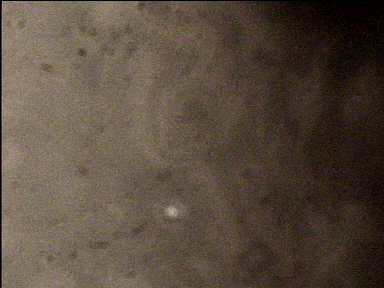
\includegraphics[width=0.7\columnwidth]{mapping_1steps_startpoint}
\caption[MH2-Q3-210 line mapping start position]{Sample MH2-Q3-210 B2 Line mapping end position. Picture is from the camera inserted into the detection path by use of a flip mirror, and sample illuminated by white light. The bright spot is reflections from the pumping laser.}
\label{fig:mapping_1steps_startpoint}%
\end{figure}


\begin{figure}[H]
\centering
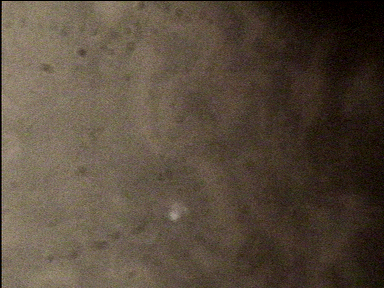
\includegraphics[width=0.7\columnwidth]{mapping_1steps_endpoint}
\caption[MH2-Q3-210 line mapping start position]{Sample MH2-Q3-210 B2 Line mapping start position. Picture is from the camera inserted into the detection path by use of a flip mirror, and sample illuminated by white light. The bright spot is reflections from the pumping laser.}
\label{fig:mapping_1steps_endpoint}%
\end{figure}

\begin{figure}[H]
\centering
\includegraphics[width=0.7\columnwidth]{MH2-mapping-small_steps-20s}
\caption[MH2-Q3-210 line mapping]{Sample MH2-Q3-210 B2 pumped with 170mW at 14K line map using 10 small steps.}
\label{fig:MH2-mapping-small_steps-20s}%
\end{figure}






Positions 1-20 has en equally large distance in between them, with position 1 in figure \ref{fig:mapping_5steps_startpoint} and position 20 in figure \ref{fig:mapping_5steps_endpoint}.

\begin{figure}[H]
\centering
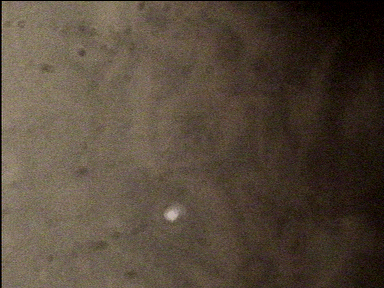
\includegraphics[width=0.7\columnwidth]{mapping_5steps_startpoint}
\caption[MH2-Q3-210 line mapping start position]{Sample MH2-Q3-210 B2 Line mapping end position. Picture is from the camera inserted into the detection path by use of a flip mirror, and sample illuminated by white light. The bright spot is reflections from the pumping laser.}
\label{fig:mapping_5steps_startpoint}%
\end{figure}


\begin{figure}[H]
\centering
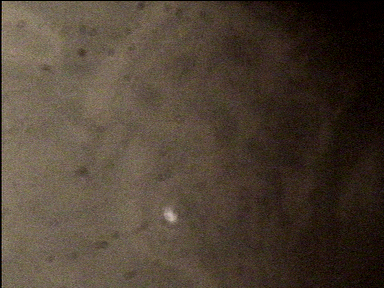
\includegraphics[width=0.7\columnwidth]{mapping_5steps_endpoint}
\caption[MH2-Q3-210 line mapping start position]{Sample MH2-Q3-210 B2 Line mapping start position. Picture is from the camera inserted into the detection path by use of a flip mirror, and sample illuminated by white light. The bright spot is reflections from the pumping laser.}
\label{fig:mapping_5steps_endpoint}%
\end{figure}

\begin{figure}[H]
\centering
\includegraphics[width=0.7\columnwidth]{MH2-mapping-5_small_steps-20s}
\caption[MH2-Q3-210 line mapping]{Sample MH2-Q3-210 B2 pumped with 170mW at 14K line map using 20 steps exactly 5 times larger than in figure \ref{fig:MH2-mapping-small_steps-20s}.}
\label{fig:MH2-mapping-5_small_steps-20s}%
\end{figure}



\clearpage
\subsection{Results analysis}

Comparison plots have been slightly filtered using weak Savitzky-Golay filtering to reduce white noise components for easier comparison. The line map and bar plots are without this filtering.

\subsubsection{Comparing different locations on sample R6-Q3-210}


\begin{figure}[H]
\centering
\includegraphics[width=0.7\columnwidth]{R6_comparisons}
\caption[R6-Q3-210 comparisons]{Comparison of different locations on sample R6-Q3-210 A from results in figure \ref{fig:R6-Area3_clean_area-20s}, \ref{fig:R6-Area1_dislocation_line-20s}, and \ref{fig:R6-Area2_dislocation_dot-20s}.}
\label{fig:R6_comparisons}%
\end{figure}

\begin{figure}[H]
\centering
\includegraphics[width=0.7\columnwidth]{R6_comparisons_Darea}
\caption[R6-Q3-210 comparisons close]{A closer look on differences in R6-Q3-210 A from graph in figure \ref{fig:R6_comparisons} }
\label{fig:R6_comparisons_Darea}%
\end{figure}

\begin{figure}[H]
\centering
\includegraphics[width=0.7\columnwidth]{R6_comparisons_TO}
\caption[R6-Q3-210 comparisons close]{A closer look on differences in R6-Q3-210 A from graph in figure \ref{fig:R6_comparisons} }
\label{fig:R6_comparisons_TO}%
\end{figure}

\begin{figure}[H]
\centering
\includegraphics[width=0.7\columnwidth]{R6_comparisons_I0}
\caption[R6-Q3-210 comparisons close]{A closer look on differences in R6-Q3-210 A from graph in figure \ref{fig:R6_comparisons} }
\label{fig:R6_comparisons_I0}%
\end{figure}


The strong TO line and its replicas, has relative intensities similar to those found in \cite{dean67}. Low impurity levels  in the sample allows for comparisons with intrinsic characteristics from \cite{dean67} (figure \ref{fig:SiPL}). Comparing figure \ref{fig:SiPL} with the results from R6 show TO + 2 Zone center phonon at 0.968~eV, TO + Zone center phonon at 1.0315~eV, intervalley phonon replicas around 1.07~eV, TO at 1.097~eV and TA at 1.365~eV. It is also possible that the peak at 1.54~eV is the ideally forbidden no phonon peak, but it is very close to the noise floor, and cannot be unequivocally identified. 

TO + Zone center phonon line have 7~\% relative intensity to TO in \cite{dean67}, when pumped with 7~W from a mercury arc on to an etched surface of intrinsic silicon. The relative intensity of TO + Zone center phonon line is \~6~\% for both the dislocation line, and defect dot. This peak at 1.092~eV is attributed to the TO phonon assisted Si:B bound excitons \cite{sauer73}. The Si:B free exciton would be at 1.150~eV, with 10\% intensity relative to the TO. This line could be present, by judgning the R6 results, however due to the noise level, it is hard to know for sure, but the relative intensities would be in the same order of magnitude as in \cite{sauer73}, if it is in fact the free exciton line.


\cite{tajima78} describe a relation between B$^{TO}$(BE)/I$^{TO}$(FE). The ratio in R6 is close to 0.1, which in \cite{tajima78} correspond to N$_A$-N$_D\approx$5$\cdot$10$^{11}$~cm$^{-3}$. R6 is in the order of 10$^{16}$~cm$^{-3}$, and with excitation intensity (150~mW in \cite{tajima78}), and temperature (liquid helium temperatures in \cite{tajima78}) being similar, there is clearly some mismatch between the samples. Other differences is \cite{tajima78} using an Ar ion laser, and having as spot size of 1~mm. This should, however, not affect the ratio in between the two lines, unless the smaller volume give rise to other types of recombination, like electron-hole drops, or non radiative recombination. One possible explanation is that \cite{tajima78} where looking at compensated high purity CZ-Si and FZ-Si, and that the relation is invalid for mc-Si. Specifically \cite{drozdov76} report a decrease in bound exciton intensities when nearing dislocation areas, which could account for the mismatch to results in \cite{tajima78}. Temperature will also influence this line such that higher temperatures lead to a smaller bound exciton luminescence. This temperature behavior is shown in figure \ref{fig:MH2-B2-Area5-tempereatures-clean_area-30s}, on sample MH2.


There are more lines present, that does not relate to intrinsic silicon, like the line at 1.0~eV. In addition, there is an increased intensity of TO + 2 zone center phonons which is expected to be 1~\% of the TO line \cite{dean67}. But this appear to be 7~\% in the R6 dislocation line , and 3~\% in the R6 defect dot. These are likely to originate from dislocations. D3 and D4 are known to appear at 0.934~eV and 1.00~eV respectively at 4.2~K in CZ-Si \cite{drozdov76}. D4 has not been observed without D3, and vice versa, and D3 is considered to be a phonon replica of D4 \cite{kveder95}. In addition, \cite{tajima95} report a broad background emission reaching from 0.9-1.0~eV with D3 and D4 present. In the R6 results, on the defect dot, there's signs of D3 and D4 lines at 0.95~eV, and 1.0~eV respectively. This corresponds to measurements on mc-Si with a temperature of 77K, from \cite{tarasov00}, which reports a shift in the energies when comparing CZ-Si and mc-Si. The D3 line is more intense than D4, which suggest that there is additional luminescence present for this wavelength not attributed to D3.

If, in fact, it is the D3 and D4 lines in the result, D1 and D2, which also are attributed to dislocation areas, are completely missing. \cite{kitler02} state that a relatively low contamination level of dislocations in the order of 10 impurity atoms/mm of the dislocation length produces D1 defect luminescence at room temperature. \cite{arguirov07} state that D1 and D2 are most probably caused by the interaction of the dislocations with metallic impurities. This is a probable reason for the missing D1 and D2 lines, due to the low level of metallic impurities in R6.

When pumping at lower intensities, the relative intensity of D3' and D4' compared to TO is higher. This is most likely caused by the D3 and D4 lines reaching saturation for high intensities, effectively halting the rise of these bands for higher pumping light intensities. These lines are also considerably smaller for a defect free area, where they are likely to arise from defects below the surface. 

There are two peaks observed at 1.04~eV and 0.98~eV. The 0.98~eV line, is only distinguishable in figure \ref{fig:R6-A-Area4-intensities-grain_boundary-30s}, but is likely to be present in the other results as well, based on the shape of the dislocation related luminescence, which has a contribution to the photoluminescence in between D3 and D4. These lines are known as R1BB and R2BB \cite{arguirov02,arguirov03}. \cite{arguirov03} (figure \ref{fig:R1BB} in appendix) observed these lines in FZ-Si as well as mc-Si, and suggest that they are most probably phonon replicas of the band edge emission with 1, and 2 phonons respectively. This fits well with I$^{TO+0^\Gamma}$ and I$^{TO+20^\Gamma}$ found in intrinsic silicon in \cite{dean67}, except for the results in \ref{fig:R6-A-Area4-intensities-grain_boundary-30s} where the 0.98~eV peak is considerably larger than any luminescence at 1.04~eV. This can be due to a defect or impurity present in the grain boundary besides the dislocation lines. There is a known line caused by a carbon-carbon complex at 0.969~eV \cite{davies88}. Carbon is known to be unevenly distributed in mc-Si \cite{teng09}. It is possible, that the grain boundary act as a impurity center, where impurity atoms gather, and therefor have a higher impurity concentration than other areas in the sample. The C-C complex is known to saturate at a value proportional to static substitutional carbon atoms combined with interstitial carbon atoms \cite{weber86}, which fits the behavior of this line which appear to saturate for higher excitation intensities. 

The two peaks observed above 1.16~eV observed in some of the results, are of unknown origin. The background noise, and dark current has been subtracted, however, the fact that these peaks have the same intensity and shape for different pumping intensities, and have energies above the silicon band gap, suggest that these are in fact not photoluminescence signal, but noise added by the system, or a change in the background noise emission. It is possible that the background noise changed after the noise was measured, causing these peaks.


\subsubsection{Comparing different locations on sample ES1-Q3-201}

Room temperature does not reveal any luminescence, except the main TO line. The TO line has substantial broadening due to the temperature. Defect lines would appear below the TO line, but are not present.


\begin{figure}[H]
\centering
\includegraphics[width=0.7\columnwidth]{ES1_comparisons}
\caption[ES1-Q3-201 comparisons]{Comparison of different locations on sample ES1-Q3-201 C from results in figure \ref{fig:ES1-Area1_dislocation_free-10s}, \ref{fig:ES1-Area4_dislocation_line-60s}, \ref{fig:ES1-Area2_dislocation_spot-10s}, and \ref{fig:ES1-Area3_grain_boundary_60s}. }
\label{fig:ES1_comparisons}%
\end{figure}

\begin{figure}[H]
\centering
\includegraphics[width=0.7\columnwidth]{ES1_comparisons_Darea}
\caption[ES1-Q3-201 comparisons close]{A closer look on differences in ES1-Q3-201 C from graph in figure \ref{fig:ES1_comparisons} }
\label{fig:ES1_comparisons_Darea}%
\end{figure}

\begin{figure}[H]
\centering
\includegraphics[width=0.7\columnwidth]{ES1_comparisons_TO}
\caption[ES1-Q3-201 comparisons close]{A closer look on differences in ES1-Q3-201 C from graph in figure \ref{fig:ES1_comparisons} }
\label{fig:ES1_comparisons_TO}%
\end{figure}

\begin{figure}[H]
\centering
\includegraphics[width=0.7\columnwidth]{ES1_comparisons_I0}
\caption[ES1-Q3-201 comparisons close]{A closer look on differences in ES1-Q3-201 C from graph in figure \ref{fig:ES1_comparisons} }
\label{fig:ES1_comparisons_I0}%
\end{figure}


Known intrinsic values are present, and recognized as I$^{TO+20^\Gamma}$[0.968~eV], I$^{TO+0^\Gamma}$[1.0315~eV], I$^{TO}$[1.097~eV], and I$^{TA}$[1.1365~eV]. In addition there are some expected, less defined luminescence at the TO intervalley phonon replica energies of 1.151~eV and 1.074~eV, and intervalley I$^{TO+0^\Gamma}$ replica energy at 1.013~eV. No phonon luminescence at 1.1545~eV seems to disappear in the area of grain boundary and dislocation line. A possible explanation for this, is that the emitted photons carry enough energy to excite a new electron-hole pair. Due to the geometrical properties of dislocation etched line and grain boundary, there is an etch pit with less atoms blocking the excitation laser, compared to the case of a perfect crystal structure. This would result in the laser penetrating deeper into the sample, and the photons are emitted from a deeper region of the sample and are less likely to be emitted with a direct path out of the sample.

%%%%%%%%%%%%%%%%%%%%%%%%%%%%% why??
%Dislocation related luminescence does not show up as individual luminescence. 

Phosphorus no phonon line is observed at 1.1496~eV in \cite{dean67}. This line should be accompanied by a TO phonon assisted line at 1.0916~eV with three times the intensity. These are not resolved in the ES1 results, but given the strong bound exciton peak, it's likely that it is present. Boron has a similar characteristic, with the no phonon line at 1.1503~eV, and TO phonon assisted line at 1.0924~eV. The no phonon line should have around 0.5\% of the B$^{TO}$ line, which is a considerably larger ratio than that of the P$^{TO}$ line \cite{dean67}. Boron and phosphorus lines are indistinguishable from each other, but both are likely to influence the luminescence. 


As expected, there are no C-O line present. As for Fe bound with B, a sharp line a 1.068~eV should be present \cite{mohring83}. Even though it could appear like this line is present, it is more likely that this is an artifact from noise, as the same sharp peak shape can be observed in different parts of the spectra known to contain nothing but noise. Based on the repeating on this peak, it is possible that the mean dark current noise has shifted, in regards to intensity for some pixels, compared to the measured mean dark current which is subtracted. An example which shows that the mean dark current noise has shifted, is the repeating artifacts from 0.7~eV to 0.9~eV. As the spectra consist of several glued together spectra, the artifact is repeating itself. These spectra has been glued together with some overlap, so that one side of the spectra has been removed. The rising intensities at 1.3~eV for the red line, show the non-overlapping part of the spectra. For lower energies, these pixels have been disregarded, and replaced by overlap except for the last interval.

Pumping at lower intensities, a new band is observed with peak value at 1.04~eV. Band edge emission phonon replica can not explain this band. According to \cite{dean67}, a phonon replica of the TO band, have 7\% of relative intensity compared to TO at these energies, which prove that this luminescence originates from something else. It is clearly a band with lower energy levels than the band emission, making it the lowest, most probable place for electrons energies to occupy. It also appear to saturate, which means that there is a limited amount of availible states, consistent with a defect band. The bound exciton also decrease in relative intensity compared to the TO line for higher excitation power. Increased temperature is known to have this effect (as seen in figure \ref{fig:MH2-B2-Area5-tempereatures-clean_area-30s}), and is a possible explanation for this behaviour, with increased local heating for higher excitation intensities.

\cite{misiuk99} observe a PL peak at 1.04~eV in oxygen implanted FZ-Si. This is presumably related to some intrinsic point defects in reactively etched silicon shown in \cite{erzgraber96}. \cite{enck69} report a line at 1.04~eV for P and B doped samples. \cite{enck69} state that this is a TO phonon assisted line, with the no phonon line at 1.1~eV, and TA assisted line a 1.08~eV. In addition, a very weak two phonon assisted line was observed at 0.98~eV in \cite{enck69}. Looking at the spectra in figure \ref{fig:ES1-C-Area5-intensities-clean_area-30s} and \ref{fig:ES1-C-Area6-intensities-grain_boundary-30s}, the relative luminescence intensities at low pumping values, is similar to those found in \cite{enck69} (figure \ref{fig:BPSiPL}), and thus attributed to the presence of both boron and phosphorous doping atoms. \cite{enck69} also observe a small shift to lower energies for the peak, when increasing pumping intensity. This is consistent with the pumping intensity variation plots of figure \ref{fig:ES1-C-Area5-intensities-clean_area-30s}, which is in a clean area, but less apparent for figure \ref{fig:ES1-C-Area6-intensities-grain_boundary-30s}, which is in the grain boundary. Particularly for higher excitation intensities, like 33.8~mW, the dislocation related bands from D4' and D3' are emerging, reducing the intensity of the 1.04~eV line, in addition to contributions from phonon replicas of the band emission. The reduction of the 1.04~eV band with increased excitation intensities is most likely due to a change in exciton lifetime. With higher intensities, the broadening of the TO line, suggest local heating is taking place, which would influence the lifetime, making the electron hole pairs recombine before reaching the defect state related to P and B atoms.





\subsubsection{Comparing different locations on sample MH2-Q3-210}

Room temperature measurements on MH2 is nearly identical to those of ES1. Substantial broadening, with respect to energies, of the TO-line, and there are no defect bands present. At 70~K, the line has a considerably smaller energy span, and other phonon assisted bands begin to emerge. However, there is still no defect lines present.

\begin{figure}[H]
\centering
\includegraphics[width=0.7\columnwidth]{MH2_comparisons}
\caption[MH2-Q3-210 comparisons]{Comparison of different locations on sample MH2-Q3-210 B2 from results in figure \ref{fig:MH2-Area1-dislocation_free-20s}, \ref{fig:MH2-Area2-dislocation_line-20s}, and \ref{fig:MH2-Area3-dislocation_dot-60s} }
\label{fig:MH2_comparisons}%
\end{figure}


\begin{figure}[H]
\centering
\includegraphics[width=0.7\columnwidth]{MH2_comparisons_Darea}
\caption[MH2-Q3-210 comparisons close]{A closer look on differences in MH2-Q3-210 B2 from graph in figure \ref{fig:MH2_comparisons} }
\label{fig:MH2_comparisons_Darea}%
\end{figure}

\begin{figure}[H]
\centering
\includegraphics[width=0.7\columnwidth]{MH2_comparisons_TO}
\caption[MH2-Q3-210 comparisons close]{A closer look on differences in MH2-Q3-210 B2 from graph in figure \ref{fig:MH2_comparisons} } 
\label{fig:MH2_comparisons_TO}%
\end{figure}

\begin{figure}[H]
\centering
\includegraphics[width=0.7\columnwidth]{MH2_comparisons_I0}
\caption[MH2-Q3-210 comparisons close]{A closer look on differences in MH2-Q3-210 B2 from graph in figure \ref{fig:MH2_comparisons} } 
\label{fig:MH2_comparisons_I0}%
\end{figure}


The no phonon line at 1.545~eV is not observed. TA, TO, BE, intervally phonon replica, and zone center phonon TO replica lines are recognized from figure \ref{fig:SiPL}. In addition, there are some luminescence around 1.0~eV, particularly below, which cannot be attributed to 2 zone center phonon TO replica alone. If this is due to D4, which can be observed at 1.0~eV, then D3 should also be observed at 0.934~eV. While it is still possible these lines contribute to the intensity, the luminescence cannot be explained by these alone, due to the asymmetrical shape. \cite{arguirov07} observe a similar behavior around D4 at 80K, and argue that it indicates residual stress leading to strong multi-phonon (two and three, such as R1BB and R2BB) mediated band-to-band luminescence rather than radiation from defects. 

When pumping MH2 at different intensities, the same impurity line at 1.04~eV as seen in ES1 is observed. However, when looking at a grain boundary in MH2, there is an additional line present at 0.99~eV. A similar line has been reported in \cite{gundel099} for 80K, accompanied by a line at 0.93~eV attributed as a phonon replica of the 0.99~eV line in areas of high stress. Crystal defects such as dislocations, grain boundaries and precipitates cause internal stress \cite{becker07}. Dislocations has also been shown to form at grain boundaries during the solidification process as a stress relief \cite{becker07}. Due to the energy positions, \cite{gundel099} suggest, that these two peaks are the same as the D3 and D4 lines. This is a possible explanation for the results in figure \ref{fig:MH2-B2-Area4-intensities-grain_boundary-30s}, but the line at 0.93~eV, if in fact it is a luminescence line, is very weak. It also does not account for the luminescence at 0.95~eV, increasing with increased excitation intensity, even though this line is likely to be related to dislocation luminescence as well.
%%%%%%%%%%%what does it mean?

Looking at the temperature plots in figure \ref{fig:MH2-B2-Area5-tempereatures-clean_area-30s}, a shift in the peak energy is observed. The B+P attributed line at 1.04~eV disappears for temperatures above 50K, and there is broadening of the band to band luminescence. At 70K, the bound exciton is no longer observed either. This clearly shows the need for having temperatures below the boiling temperature of nitrogen (77K), in order to detect and describe impurities and defects in silicon. Particularly when intending to excite the sample with low pumping intensities.

CrB$^0$ from \cite{conzelmann82} where expected at 0.8432~eV. This is not the case for MH2. Chromium not bound with boron, does not to give rise to any luminescence, and \cite{conzelmann82} did not find any chromium related signal in phosphorous doped samples. \cite{conzelmann82} state that the intensity of this line is proportional with the chromium boron pairs. This would mean that the formation of these pairs have not taken place in MH2. \cite{conzelmann82} used chromium doped (by diffusion) Si:B FZ and CZ samples stored at room temperature, to give CrB pairs time to bond. MH2 is mc-Si, and CrB pairs in MH2 have been investigated in \cite{hystad09} by measuring lifetime. No change in lifetime occurred by regards to time, which also suggest that the forming of these pairs have not taken place in MH2 to the extent that it is detectable. This implies that chromium is mostly dissolved in the silicon lattice as an interstitial specie.



%% Line plots

\begin{figure}[H]
\centering
\includegraphics[width=0.7\columnwidth]{MH2-mapping-bars-small_steps-20s}
\caption[MH2-Q3-210 line mapping]{Sample MH2-Q3-210 B2 pumped with 128~mW at 14~K line map using 10 small steps, looking at TO and BE line only from results in figure \ref{fig:MH2-mapping-small_steps-20s}.}
\label{fig:MH2-mapping-bars-small_steps-20s}%
\end{figure}



\begin{figure}[H]
\centering
\subfigure{
\includegraphics[width=.45\columnwidth]{MH2-mapping-bars-5_small_steps-20s}
\label{fig:MH2-mapping-bars-5_small_steps-20s}
}
\subfigure{
\includegraphics[width=.45\columnwidth]{MH2-mapping-bars-TOonBE-5_small_steps-20s}
\label{fig:MH2-mapping-bars-TOonBE-5_small_steps-20s}
}
\label{fig:MH2-5stepmapping}
\caption[MH2-Q3-210 line mapping]{Sample MH2-Q3-210 B2 pumped with 128~mW at 14~K line map using 20 small steps exactly 5 times larger than in figure \ref{fig:MH2-mapping-bars-small_steps-20s}. Looking at TO and BE line only from results in figure \ref{fig:MH2-mapping-5_small_steps-20s}.}
\end{figure}


The similar intensities for different small areas implies that for a small area, neither the band to band luminescence, or doping concentrations, are subject to much change. When having larger steps, there is a change in band to band luminescence corresponding to a dislocation line. Looking at the relation between the bound exciton and the TO line, \cite{tajima78} state that there is little or no change in doping atom concentrations.



\subsubsection{Comparing similar areas on different samples}


\begin{figure}[H]
\centering

\subfigure[Comparisons of a clean area]{
\includegraphics[width=0.45\columnwidth]{clean_area-20s}
\label{fig:clean_area-20s_comparison}%
}
\subfigure[Plot from figure \ref{fig:clean_area-20s_comparison} in greater detail]{
\includegraphics[width=0.45\columnwidth]{clean_area-20s_zoom}
\label{fig:clean_area-20s_zoom_comparison}%
}
\caption[Comparisons in a clean area]{Results from figure \ref{fig:R6-Area3_clean_area-20s},\ref{fig:ES1-Area1_dislocation_free-10s}, and \ref{fig:MH2-Area1-dislocation_free-20s} where results in figure \ref{fig:ES1-Area1_dislocation_free-10s} are multiplied by 2, to account for 10s integration time compared to 20s.}
\label{fig:comparisons_of_a_clean_area}
\end{figure}

Both ES1 and MH2 have more luminescence at 1.04~eV, and at the bound exciton relative to TO, compared to R6. This is expected, due to the lower amount of P and B atoms in R6.

\begin{figure}[H]
\centering

\subfigure[Comparisons in a defect dot]{
 \includegraphics[width=0.45\columnwidth]{dislocation_dot-20s}
 \label{fig:dislocation_dot-20s_comparison}%
}
\subfigure[Plot from figure \ref{fig:dislocation_dot-20s_comparison} in greater detail]{
 \includegraphics[width=0.45\columnwidth]{dislocation_dot-20s_zoom}
 \label{fig:dislocation_dot-20s_zoom_comparison}%
}
\caption[Comparisons in a defect dot]{Results from figure \ref{fig:R6-Area2_dislocation_dot-20s},\ref{fig:ES1-Area2_dislocation_spot-10s}, and \ref{fig:MH2-Area3-dislocation_dot-60s} where results in figure \ref{fig:ES1-Area2_dislocation_spot-10s} are multiplied by 2, to account for 10s integration time compared to 20s. }

\label{fig:comparisons_in_a_dislocation_dot}
\end{figure}


Compared to MH2, ES1 have a fairly intense bound exciton line at 1.092~eV. This corresponds to a higher concentration of boron and phosphorus atoms according to \cite{tajima78}. The ratio is different on different parts of the sample, which could mean that the doping atoms are unevenly distributed. It could also mean that the excitons at defect locations are more subject to interaction with defect characteristics, than the TO line. This behavior was reported in \cite{drozdov76}, which state that the series of bound exciton lines decrease sharply in intensity in areas of dislocations. This could mean that the ES1 sample, has less dislocations in the measured areas than MH2, based on the fact that B and P concentrations should be the same for both samples. It can also be due to a higher temperature in MH2, and ES1, resulting in a weaker bound exciton line for MH2.


\begin{figure}[H]
\centering
\subfigure[Comparisons in a dislocation line]{
 \includegraphics[width=0.45\columnwidth]{dislocation_line-20s}
 \label{fig:dislocation_line-20s_comparison}%
}
\subfigure[Plot from figure \ref{fig:dislocation_line-20s_comparison} in greater detail]{
 \includegraphics[width=0.45\columnwidth]{dislocation_line-20s_zoom}
 \label{fig:dislocation_line-20s_zoom_comparison}%
}

\caption[Comparisons in a dislocation line]{Results from figure \ref{fig:R6-Area1_dislocation_line-20s},\ref{fig:ES1-Area4_dislocation_line-60s}, and \ref{fig:MH2-Area2-dislocation_line-20s} where results in figure \ref{fig:ES1-Area4_dislocation_line-60s} are multiplied by 2, to account for 10s integration time compared to 20s. }
\label{fig:comparisons_of_a_dislocation_line}
\end{figure}


It is clear that the bound exciton line in R6, compared to TO, corresponding to boron and/or phosphorous levels \cite{tajima78}, is lower than those from ES1 and MH2. This is expected, with the lower levels of doping atoms in this sample. The lines corresponding to dislocations, D3 and D4 are not well resolved, suggesting that photoluminescence from these energies are influenced by impurities as well as phonon replicas of the band edge emission. It can also mean that they are reduced due to a change in lifetime due to local heating.

An interesting observation is that the luminescence from ES1 is considerably stronger than for both R6, and MH2. This can also be confirmed by looking at the different excitation intensity plots in figure \ref{fig:ES1-C-Area5-intensities-clean_area-30s} and \ref{fig:ES1-C-Area6-intensities-grain_boundary-30s}, where the signal is detected for considerably lower excitation intensity compared to those of R6, and MH2. This would mean that the ES1 sample is if higher quality than the other two, with regards for using it in a solar cell. This is likely to be related to the increased lifetime of the ES1 sample, compared to MH2, as described in \cite{hystad09}.

MH2 have some broadening of the TO line, with respect to energy, that resemble that of higher temperature plots. Broadening on the lower energy side of the band to band luminescence can be attributed to bound excitons, but the broadening on the higher energy side is due to an increased number of phonon states. It is likely to be some local heating, when exciting the sample with high intensities. Using the theoretical shape from equation \ref{eq:to_line}, the local heating appear to be substantial, as represented in figure \ref{fig:temperature_fitting}. It is possible that the MH2 have a smaller thermal conductivity than the other samples, leading to more broadening than the other two. 

\begin{figure}[H]
\centering
\includegraphics[width=\columnwidth]{MH2_Temperature_fitting}%
\caption{Temperature fitting using equation \ref{eq:to_line} on MH2 results from line map in figure \ref{fig:MH2-mapping-small_steps-20s}}%
\label{fig:temperature_fitting}%
\end{figure}

Looking at the different temperature plots in figure \ref{fig:MH2-B2-Area5-tempereatures-clean_area-30s} done in a clean area, using 16~mW compared to 128~mW excitation intensity suggest that any defect band would rapidly loose intensity when reaching 70~K. This is consistent with the results in figure \ref{fig:MH2-70K}, which is done using 128~mW excitation intensity at 70~K, not showing any strong defect lines. 

Silicon is known to get a smaller band gap when increasing temperature \cite{alex96}. This change is however quite small for 0-70~K. There is a substantial broadening of the phonon assisted recombination with regards to energy as seen in figure \ref{fig:MH2-B2-Area5-tempereatures-clean_area-30s}. By using the theoretical shape for the TO line from \cite{davies88}, a substantial local heating is revealed. Looking at the plots from all of the samples, using different excitation intensities, a broadening of the TO lines can be observed when increasing the excitation intensity.

\cite{davies88} state that with excitation powers of 1.5~W/mm$^2$, with the sample at 20~K, it is heated by less than 0.5~K. With a spot size of around 2~$�$m, there are bound to be issues regarding local heating. Single crystal silicon has maximum thermal conductivity at 30~K, of around 4~W/mmK \cite{glassbrenner64}. A spot diameter of 2$�$m, with 128~mW excitation energy, as in figure \ref{fig:temperature_fitting}, corresponds to 40~kW/mm$^2$. As silicon has an indirect band gap, nearly all the excitation light intensity, not reflected back, is absorbed as heat. 

Local heating is a major problem, as it broadens the luminescence with regards to energy, decrease peak strength by contributing to non-radiative recombination, and lowers the band gap. Looking at figure \ref{fig:MH2-B2-Area5-tempereatures-clean_area-30s}, showing the luminescence at increasing temperatures, using the same excitation intensity, clearly show how heat is undesirable. Using lower excitation intensity and longer integration times, can overcome parts of the problem with local heating, but then the signal is likely to be close to the noise floor, making it hard to detect. This puts micro photoluminescence at a disadvantage compared to macro photoluminescence.

Local heating is also a possible explanation for the mismatch in P and B concentrations in regards to the bound exciton line, compared to the relation to TO line found in \cite{tajima78}. With increasing temperature, the bound exciton intensity decrease more rapidly, than the TO line, as showed in figure \ref{fig:MH2-B2-Area5-tempereatures-clean_area-30s}, invalidating the corresponding B and P concentration relation found in \cite{tajima78}. In addition, the dislocation related luminescence is known to decrease with increasing temperatures \cite{arguirov02}, and could explain the poorly resolved luminescence lines attributed to dislocations.

%\begin{figure}[H]
%\centering
%\includegraphics[width=\columnwidth]{TO_comparisons}
%\caption[Comparison or relative strength]{Comparison of relative strength of known characteristics to TO line}
%\label{fig:TO_comparisons}%
%\end{figure}


%% Total luminescence graphs

%R6
\begin{figure}[H]
\subfigure[Area 4 in figure \ref{fig:R6-Q3-210-A_enlarged} - Grain boundary]{
 \includegraphics[width=.45\columnwidth]{R6-A-Area4-total_luminescence-grain_boundary-30s}%
 \label{fig:R6_tot_lum_grain}%
}
\subfigure[Area 4 in figure \ref{fig:R6-Q3-210-A_enlarged} - Clean area]{
 \includegraphics[width=.45\columnwidth]{R6-A-Area5-total_luminescence-clean_area-30s}
 \label{fig:R6_tot_lum_clean}
}
\label{fig:R6_total_luminescence}
\caption{Total luminescence from sample R6 A, as a function of excitation intensity.}%
\end{figure}


%ES1
\begin{figure}[H]
\subfigure[Area 6 in figure \ref{fig:ES1-Q3-201-C_enlarged} - Grain boundary]{
 \includegraphics[width=.45\columnwidth]{ES1-C-Area6-total_luminescence-grain_boundary-30s}%
 \label{fig:ES1_tot_lum_grain}%
}
\subfigure[Area 5 in figure \ref{fig:ES1-Q3-201-C_enlarged} - Clean area]{
 \includegraphics[width=.45\columnwidth]{ES1-C-Area5-total_luminescence-clean_area-30s}
 \label{fig:ES1_tot_lum_clean}
}
\label{fig:ES1_total_luminescence}
\caption{Total luminescence from sample ES1 C, as a function of excitation intensity.}%
\end{figure}


%MH2
\begin{figure}[H]
\subfigure[Area 4 in figure \ref{fig:MH2-Q3-210-B2_enlarged} - Grain boundary]{
 \includegraphics[width=.45\columnwidth]{MH2-B2-Area4-total_luminescence-grain_boundary-30s}%
 \label{fig:MH2_tot_lum_grain}%
}
\subfigure[Area 5 in figure \ref{fig:MH2-Q3-210-B2_enlarged} - Clean area]{
 \includegraphics[width=.45\columnwidth]{MH2-B2-Area5-total_luminescence-clean_area-30s}
 \label{fig:MH2_tot_lum_clean}
}
\label{fig:MH2_total_luminescence}
\caption{Total luminescence from sample MH2 B2, as a function of excitation intensity.}%
\end{figure}


Looking at the total luminescence coming from the samples, it shows that the grain boundaries does not relate linearly with regards to emitted luminescence compared to excitation intensity, particularly for ES1 and MH2. This means that the recombination is influenced by defects and impurities in the grain boundary leading to either increased, or decreased non-radiative recombination for different excitation intensities. This, in turn, mean that the lifetime of electron hole pairs are changing in the grain boundary with respects to excitation intensity. Much more so than for a clean area, which are closer to a linear response. Another influence for this behavior is local heating from the excitation laser, leading to a change in lifetime.


\subsection{Further work}

It is clear that ES1 has more radiative recombination, than the other two samples. It is assumed that the increased lifetime in ES1, compared to MH2 is related, but the reason is still not clear, due to the small differences in between these two samples. Further studies are needed in order to determine why the ES1 appear to be of higher photovoltaic quality than both MH2 and R6. 

It is likely that there is a substantial local heating when using high excitation intensity in micro photoluminescence. The effects of local heating in micro photoluminescence needs to be analyzed more closely, in order to minimize the impact it has on the result.
\clearpage
\section{Discussion}


%\clearpage
%\input{diskusjon}
%\clearpage
%\input{konklusjon}
%\input{test}

% Referanse list
\clearpage
%\bibliographystyle{plain} % Alfabetic list
\bibliographystyle{ieeetr} % To number the references in order of appearance, rather than alphabetical order use ieeetr
\nocite{*} % List all references, including unused ones
\bibliography{bibliography} % bibliography.bib

% Appendixes
\clearpage
\appendix % Start of appendix sections
\label{appendix:tabeller}
\appendix

\section{Silicon energy bands}

\addtolength{\hoffset}{-1.5cm}
\begin{small}
\begin{center}
\begin{longtable}{|c|c|c|c|c|}

% Header for first page
\hline 
\multicolumn{1}{|c|}{\textbf{Energy}} & 
\multicolumn{1}{c|}{\textbf{Name}} & 
\multicolumn{1}{c|}{\textbf{Temp.}} & 
\multicolumn{1}{c|}{\textbf{Impurity / Defect}} & 
\multicolumn{1}{c|}{\textbf{Observed in}} \\ \hline
\endfirsthead


% Header for page 2 3 4 etc.
\multicolumn{5}{c}{{\bfseries \tablename\ \thetable{} -- continued from previous page}} \\
\hline 
\multicolumn{1}{|c|}{\textbf{Energy}} & 
\multicolumn{1}{c|}{\textbf{Name}} & 
\multicolumn{1}{c|}{\textbf{Temp.}} & 
\multicolumn{1}{c|}{\textbf{Impurity / Defect}} & 
\multicolumn{1}{c|}{\textbf{Observed in}} \\ \hline
\endhead

% Table footer on first pages
\hline \multicolumn{5}{|r|}{{Continued on next page}} \\ \hline
\endfoot

% Table footer on last page
\caption{Silicon energy bands}
\label{energy_bands}
\endlastfoot


\hline
0.735eV & ZPL & 22K & Fe contamination & \cite{calao88} \\ \hline
0.745eV & C-N & & Carbon-Nitrogen complex & \cite{davies88} \\ \hline
0.76-0.8eV & Defect & 290K & Dislocation with low contamination & \cite{tarasov00} \cite{tarasov01} \cite{arguirov06} \\ \hline
0.77-0.78eV & D$_b$ & 4.2-295K & Oxygen impurity band & \cite{tajima95} \cite{inoue07} \\ \hline
0.77eV & P line & 12K & C-O complex related & \cite{davies88} \cite{binetti08} \\ \hline
0.780eV & CrB$^{0 \Gamma }$ & 4.2K & CrB$^0$ phonon replica & \cite{conzelmann83} \\ \hline
0.79eV & C-O & 12K & Carbon-Oxygen complex & \cite{davies88} \cite{binetti08} \\ \hline
0.80eV & D1' & 77K & Dislocations \footnotemark[1] & \cite{tarasov00} \cite{tarasov01} \\ \hline
0.812eV & D1 & 4.2K & Dislocation related line \footnotemark[1] & \cite{drozdov76} \cite{sauer85} \cite{arguirov03} \\ \hline
0.8160 & CrB$^2$ & 4.2K & Cr-B excitation of local vibrations & \cite{conzelmann83} \\ \hline
0.8402 & CrB$^1$ & 4.2K & Cr-B excitation of local vibrations & \cite{conzelmann83} \\ \hline
0.8432eV & CrB$^0$ & 4.2K & Cr-B pair no-phonon & \cite{conzelmann83} \\ \hline
0.875eV & C-Ga & & Carbon-Gallium complex & \cite{davies88} \\ \hline
0.875eV & D2 & 4.2K & Dislocation related line \footnotemark[1] & \cite{drozdov76} \cite{sauer85} \cite{arguirov03} \\ \hline
0.89eV & D2' & 77K & Dislocations \footnotemark[1] & \cite{tarasov00} \cite{tarasov01} \\ \hline
0.8-0.9eV & D$_{a1}$ & 11K & Broad background emission under D1/D2 & \cite{tajima95} \\ \hline
0.91eV & H-line & 12K & C-O complex related & \cite{davies88} \cite{binetti08} \\ \hline
0.93eV & H-line & 12K & C-O complex related & \cite{davies88} \cite{binetti08} \\ \hline
0.934eV & D3 & 4.2K & Dislocations \footnotemark[2] & \cite{drozdov76} \cite{sauer85} \cite{arguirov03} \\ \hline
0.95eV & D3' & 77K & Dislocations \footnotemark[2] & \cite{tarasov00} \cite{tarasov01} \\ \hline
0.953eV & D5 & 4.2K & Straight dislocations & \cite{sauer85} \cite{weronek91} \\ \hline
0.968eV & I$^{TO+20^\Gamma}$ & 26K & TO + 2 Zone center phonon & \cite{dean67} \\ \hline
0.969eV & C-C & & Carbon-Carbon complex & \cite{davies88} \\ \hline
0.98eV & R2BB & 80K & Two phonon replica of band edge emission & \cite{arguirov03} \\ \hline
0.9-1.0eV & D$_{a2}$ & 11K & Broad background emission under D3/D4 & \cite{tajima95} \\ \hline
1.000eV & D4 & 4.2K & Dislocations \footnotemark[2] & \cite{drozdov76} \cite{sauer85} \cite{arguirov03} \\ \hline
1.00eV & D4' & 77K & Dislocations \footnotemark[2] & \cite{tarasov00} \cite{tarasov01} \\ \hline
1.0089eV & FeB$^0$(TO) & 6K & Fe-B pair phonon replica & \cite{mohring83} \\ \hline
1.0126eV & D6 & 4.2K & Stacking faults & \cite{sauer85} \cite{weronek91} \\ \hline
1.013eV & I$^{TO+0^\Gamma+IV^a}$ & 26K & $TO+0^ \Gamma +IV^a$ phonon & \cite{dean67} \\ \hline
1.014eV & Cu$_0$ & 4.2K & Copper doping & \cite{weber82} \cite{weronek91} \\ \hline
1.018eV & W/I1 & & Radiation damage & \cite{davies88} \\ \hline
1.0315eV & I$^{TO+0^ \Gamma}$ & 26K & TO + Zone center phonon & \cite{dean67} \\ \hline
1.04eV & R1BB & 80K & One phonon replica of band edge emission & \cite{arguirov03} \\ \hline
1.045eV & Q & & 4-Li atom complex & \cite{davies88} \\ \hline
1.0504eV & FeB$^{2}$ & 6K & Fe-B pair contamination & \cite{mohring83} \\ \hline
1.051eV & I$^{TO+IV^b}$ & 26K & Inter valley phonon replica & \cite{dean67} \\ \hline
1.0595eV & FeB$^{1}$ & 6K & Fe-B pair contamination & \cite{mohring83} \\ \hline
1.0692eV & FeB$^{0}$ & 6K & Fe-B pair no phonon & \cite{mohring83} \\ \hline
1.074eV & I$^{TO+IV^a}$ & 26K & Inter valley phonon replica & \cite{dean67} \\ \hline
1.078 & EHD & 4.2K & Electron Hole Droplet dislocation-area & \cite{drozdov03} \\ \hline
1.082eV & EHD$_{TO}$ & 4.2K & Electron Hole Droplet dislocation-free & \cite{hammond75} \cite{drozdov03} \cite{satoshi04} \\ \hline
1.0835eV & In$^{TO}$ & 30K & Indium doping TO & \cite{dean67} \\ \hline
1.0888eV & Bi$^{TO}$ & 15K & Bismuth doping TO & \cite{dean67} \\ \hline
1.0902eV & Al$^{TO}$ & 30K & Aluminum doping TO & \cite{dean67} \\ \hline
1.0907eV & As$^{TO}$ & 15K & Arsenic doping TO & \cite{dean67} \\ \hline
1.0907eV & Ga$^{TO}$ & 15K & Gallium doping TO & \cite{dean67} \\ \hline
1.0916eV & P$^{TO}$ & 15K & Phosphorus doping TO & \cite{dean67} \\ \hline
1.092eV & BE1 & 4.2K & Bound exciton & \cite{drozdov76} \\ \hline
1.0921eV & Sb$^{TO}$ & 15K & Antimony doping TO & \cite{dean67} \\ \hline
1.0970eV & I$^TO$/FE & 26K & Transversal Optical/Free exciton & \cite{dean67} \cite{hammond75} \cite{drozdov03} \\ \hline
1.0924eV & B$^{TO}$ & 15K & Boron doping TO & \cite{dean67} \\ \hline
1.093eV & B$_{TO}$ & 4.2K & TO phonon replica of Boron bound exciton & \cite{sugimoto07} \cite{inoue07} \\ \hline
1.1365eV & I$^TA$/LO/FE & 26K & Transversal Acoustic/Longitudinal/FE & \cite{hammond75} \cite{dean67} \\ \hline
1.1545eV & I$^0$ & 26K & No phonon & \cite{dean67} \\ \hline

%1.25eV? EHD$^{TO}$ \cite{sauer85}
%1.26eV? Fe$^{TO}$ \cite{sauer85}
%BE \cite{inoue07}

\end{longtable}
\end{center}
\end{small}

\footnotetext[1]{D1 and D2:	It has been argued that they originate in electronic transition at the geometrical kinks on dislocations \cite{suezawa83}, point defects \cite{sauer85} and impurities \cite{higgs91} and/or from the reaction products of dislocations \cite{sekiguchi95}.}
	
\footnotetext[2]{D3 and D4 lines is generally thought to be related to electronic transition within dislocation cores \cite{kveder95}. In addition, it has been suggested that the D3 line most likely is a phonon-assisted replica of D4 \cite{kveder95}.
}


%%%%%%%%%%%%%%%%%%%%%%%%%%%%%%%
\clearpage
\section{Sample types and procedures}

\begin{figure}[H]
\centering
\includegraphics[width=15cm]{n-type_Si_spectra_dean67}
\caption{Low doped ($2\cdot10^{14}cm^{-3}$ P atoms) n-type Si PL specter from \cite{dean67}}%
\label{fig:SiPL}%
\end{figure}

\begin{figure}
\centering
\includegraphics[width=15cm]{boron_Si_spectra_dean67}
\caption{Boron doped ($6\cdot10^{16}cm^{-3}$) Si PL specter from \cite{dean67}}%
\label{fig:boronSiPL}%
\end{figure}


\begin{figure}
\centering
\includegraphics[width=15cm]{iron_diffused_Si_spectra}
\caption{Iron diffused Si sample at two different temperatures from \cite{calao88}}%
\label{fig:FeSiPL}%
\end{figure}


\begin{figure}
\centering
\includegraphics[width=15cm]{iron_diffused_boron_doped_Si_spectra}
\caption{Iron diffused boron doped Si sample from \cite{mohring83}}%
\label{fig:FeBSiPL}%
\end{figure}

\begin{figure}
\centering
\includegraphics[width=15cm]{CrB_Si_spectra}
\caption{Chromium diffused Boron doped Si sample from \cite{conzelmann83}}%
\label{fig:CrBSiPL}%
\end{figure}


\addtolength{\hoffset}{+1.5cm}
\begin{center}
\begin{sidewaystable}%
\small \begin{tabular}{|c|c|m{3cm}|m{4cm}|m{4cm}|m{2cm}|}

% Header for first page
%\hline 
%\multicolumn{1}{|c|}{\textbf{Ref.}} & 
%\multicolumn{1}{c|}{\textbf{Sample type}} & 
%\multicolumn{1}{c|}{\textbf{Excitation process}} & 
%\multicolumn{1}{c|}{\textbf{Area}} & 
%\multicolumn{1}{c|}{\textbf{Surface process}} & 
%\multicolumn{1}{c|}{\textbf{Doping}} \\ \hline
%\endfirsthead

% Header for page 2 3 4 etc.
%\multicolumn{6}{c}{{\bfseries \tablename\ \thetable{} -- continued from previous page}} \\
%\hline 
%\multicolumn{1}{|c|}{\textbf{Ref.}} & 
%\multicolumn{1}{c|}{\textbf{Sample type}} & 
%\multicolumn{1}{c|}{\textbf{Excitation process}} & 
%\multicolumn{1}{c|}{\textbf{Area}} & 
%\multicolumn{1}{c|}{\textbf{Processing}} & 
%\multicolumn{1}{c|}{\textbf{Doping}} \\ \hline\endhead

% Table footer on first pages
%\hline \multicolumn{6}{|r|}{{Continued on next page}} \\ \hline
%\endfoot

% Table footer on last page
%\endlastfoot
\hline
\textbf{Ref.} & \textbf{Sample type} & \textbf{Excitation process} & \textbf{Area} & \textbf{Processing} & \textbf{Doping} \\ \hline

\cite{sugimoto07} & mc-Si & 532nm Nd:YVO$_4$ & $0.1mW/10$ $�$m diameter & Sawing damage etched by HNO$_3$/HF & B-doped \\ \hline
\cite{tajima95} & Cz-Si & Kr ion laser 647nm & 10 \micro m &  & Undoped \\ \hline
\cite{drozdov76} & Cz-Si & Xenon lamp & 50mW on 3mm modulated at 9Hz & deformed by bending at 850$^\circ$ C & undoped, weak n and p \\ \hline
\cite{tarasov00} & mc-Si & 800nm AlGaAs laser & Pulsed 300mW / 3mm &  & Block-casting technique for Baysix \\ \hline
\cite{tarasov01} & mc-Si & 800nm AlGaAs at 140mW & & Produced by EFG & \\ \hline
\cite{arguirov03} & mc-Si and FZ-Si & Ar ion 514nm at 300mW & 100\micro m & Produced by EFG & boron doped $10^15cm^-1$ \\ \hline
\cite{sauer85} & FZ-Si & Kr-ion 647nm, Ar-ion 415nm and Nd-YAG 1064nm &  & Deformed a 650$^\circ$ C and 850$^\circ$ C & residual $10^{12}$cm$^{-3}$ boron \\ \hline
\cite{inoue07} & mc-Si & Nd:YVO 532nm & 6mW, 10$�$m diameter & Slicing damage etched off by HNO$_3$/HF & boron doped \\ \hline
\cite{conzelmann83} & FZ-Si and CZ-Si & & 50mW laser & Etched with HNO$_3$/HF. Chromium diffused & boron doped \\ \hline
\cite{mohring83} & FZ-Si & Ar$+$ 514nm & 500mW & Fe diffused & boron doped \\ \hline
\cite{calao88} & FZ-Si & Argon laser & & Fe diffusion & undoped \\ \hline
\cite{weber82} & & Ar$^+$ 514nm at 1.5W & & & Cu doped \\ \hline
\cite{weronek91} & FZ-Si & Ar$^+$ 514nm & & Heated above a Bunsen burner & Doped with Cu and/or Fe \\ \hline
\cite{binetti08} & mc-Si & & 6W/cm$^2$ & Polished by HNO$_3$/HF & Undoped \\ \hline
\cite{dean67} & CZ-Si & 200W mercury arc ~2.5eV & & & Undoped and doped \\ \hline
\cite{drozdov03} &  & Ar$^+$ or Kr$^+$ laser 0.6W & 0.8mm diameter & Dislocations by bending at ~700$^ \circ$C & phosphorus doped \\ \hline

\end{tabular}

\caption{Sample types and procedures}
\label{tab:sample_types}

\end{sidewaystable}
\end{center}



\clearpage
		\section{Abbrevations}
		
		\begin{table}[H]
\centering
\begin{tabular}{|c|c|}
\hline

		\textbf{Abbrevation} & \textbf{Description} \\ \hline
		B$_{TO}$ & TO phonon replica of the Boron bound exiton \cite{sugimoto07} \\ \hline
		BE & Bound exciton \\ \hline
		D$_a$ & Broad background emission \cite{tajima95} \\ \hline
		D$_b$ & Oxygen impurity band \cite{tajima95} \\ \hline
		CZ-Si & Czochralski processed Silicon \\ \hline
		D1	& Dislocation related line 1 \cite{drozdov76} \\ \hline
		D1' & Dislocation related line 1 for mc-Si \cite{tarasov00} \\ \hline
		D2	& Dislocation related line 2 \cite{drozdov76} \\ \hline
		D2' & Dislocation related line 2 for mc-Si \cite{tarasov00} \\ \hline
		D3	& Dislocation related line 3 \cite{drozdov76} \\ \hline
		D3' & Dislocation related line 3 for mc-Si \cite{tarasov00} \\ \hline
		D4	& Dislocation related line 4 \cite{drozdov76} \\ \hline
		D4' & Dislocation related line 4 for mc-Si \cite{tarasov00} \\ \hline
		EBIC & Electron beam induced current \cite{arguirov03} \\ \hline
		EBSP & Electron Backscatter Diffraction Pattern \cite{sugimoto07} \\ \hline
		EHD & Electron Hole Droplet	\\ \hline
		FE & Free exciton \\ \hline
		FZ-Si & Float-zone silicon \\ \hline
		EFG & Edge-define Film-fed Growth \\ \hline
		mc-Si & Multicrystalline silicon \\ \hline
		R1BB & One phonon replica of band edge emission \cite{arguirov03} \\ \hline
		R2BB & Two phonon replica of band edge emission \cite{arguirov03} \\ \hline
		SA GB & Small Angle Grain Boundary \\ \hline
		ZPL & Zero Phonon Line \cite{calao88} \\ \hline

		\end{tabular}
\caption{Abbreviations}
\label{abbreviations}
\end{table}
		
		

\clearpage

\section{Matlab code}

\subsection{Dead pixel correction}
\lstinputlisting{../Matlab/dead_pixel_correction.m}

\subsection{Dark current noise estimation removal}
\lstinputlisting{../Matlab/dark_current_noise_removal.m}

\subsection{Read result files from directory}
\lstinputlisting{../Matlab/get_result_from_dir.m}

\subsection{Remove overlap and glue intervals}
\lstinputlisting{../Matlab/matrix_align_and_glue_reverse.m}

\subsection{Filter and plot results}
\lstinputlisting{../Matlab/plot_result.m}

\end{document}